\documentclass[aspectratio=43]{beamer}

\usepackage[utf8]{inputenc}
\usepackage[czech]{babel}
\usepackage{minted}
\usepackage[font={small,it}]{caption}
\usepackage{listings}
\usepackage{tikz}
\usepackage{pgfplots}
\usepackage{bchart}
\usepackage{hyperref}
\usepackage{graphicx}

\usetheme{Boadilla}
\useinnertheme{rectangles}
\usenavigationsymbolstemplate{}

\definecolor{ctu}{HTML}{007AC2}
\definecolor{ctulight}{HTML}{1980C2}
\definecolor{ctuxlight}{HTML}{66ABD7}
\definecolor{ctuxxlight}{HTML}{C6DAF0}
\definecolor{complementary}{HTML}{FF9571}

\setbeamercolor{structure}{fg=ctu}
\setbeamercolor{headlinecolor}{fg=white,bg=ctu}
\setbeamercolor{subtitle}{fg=ctulight}
\setbeamerfont{frametitle}{series=\bfseries}
\setbeamerfont{title}{series=\bfseries}
\setbeamerfont{subtitle}{series=\mdseries}

\usemintedstyle{bw}
\setminted{
    bgcolor=ctuxxlight,
    breaklines,
    fontsize=\footnotesize
}

\setbeamertemplate{footline}{
    \leavevmode%
    \hbox{%
        \begin{beamercolorbox}[wd=.5\paperwidth,ht=2.25ex,dp=1ex,center]{author in head/foot}%
            \usebeamerfont{author in head/foot}\insertshortauthor
        \end{beamercolorbox}%
        \begin{beamercolorbox}[wd=.5\paperwidth,ht=2.25ex,dp=1ex,right]{title in head/foot}%
            \usebeamerfont{title in head/foot}\insertshorttitle\hspace*{6em}
            \insertframenumber{} / \inserttotalframenumber\hspace*{2ex}
        \end{beamercolorbox}}%
    \vskip0pt%
}

\setbeamertemplate{headline}{%
    \leavevmode%
    \hbox{%
        \begin{beamercolorbox}[wd=\paperwidth,ht=2.5ex,dp=1.125ex]{headlinecolor}%
        \end{beamercolorbox}%
    }
}

\newcommand{\backupbegin}{
    \newcounter{finalframe}
    \setcounter{finalframe}{\value{framenumber}}
}
\newcommand{\backupend}{
    \setcounter{framenumber}{\value{finalframe}}
}

\newcommand{\codeblock}[2]{
    \begin{center}
        \begin{minipage}{0.8\linewidth}
            \inputminted{#1}{#2}
        \end{minipage}
    \end{center}
}

% ============ Frontpage Info ============
\title[Simple Window Manager]{SWM -- Simple Window Manager}
\author[Jan Bína]{
    Jan Bína\\
    \scriptsize binajan2@fit.cvut.cz
}
\institute[]{
    \scriptsize
    Department of Theoretical Computer Science\\
    Faculty of Information Technology\\
    Czech Technical University in Prague
}
\date[June 2020]{\scriptsize June 2020}

\begin{document}

    \begin{frame}
        \titlepage
        \begin{center}
            
\includegraphics[scale=0.18]{img/ctulogo.pdf}
        \end{center}
    \end{frame}

    \begin{frame}{Goals}
        \begin{itemize}
            \itemsep1em
            \item design and implement a \textbf{stacking} window manager
            \item X11 Window System on Linux
            \item ICCCM and EWMH compliant
            \item virtual desktops
            \item window decorations, tiling
            \item extensibility, scriptability
            \item follow \textsc{unix} philosophy (do one thing and do it well)
        \end{itemize}
    \end{frame}

    \begin{frame}{What should window manager do?}
        \begin{itemize}
            \item manage windows
            \item {\color{gray} application launcher?}
            \item {\color{gray} custom taskbar?}
            \item {\color{gray} handle keybindings?}
            \item {\color{gray} compositing?}
            \item {\color{gray} \ldots}
        \end{itemize}
        \vspace{2em}
        \begin{table}
            \small
            \begin{tabular}{l|r}
                Window manager & Lines of code \\
                \hline
                xfwm & 41\,000 \\
                i3 & 35\,000\\
                bspwm & 12\,000\\
                swm & 5\,000
            \end{tabular}
        \end{table}
    \end{frame}

    \begin{frame}
        \begin{center}
            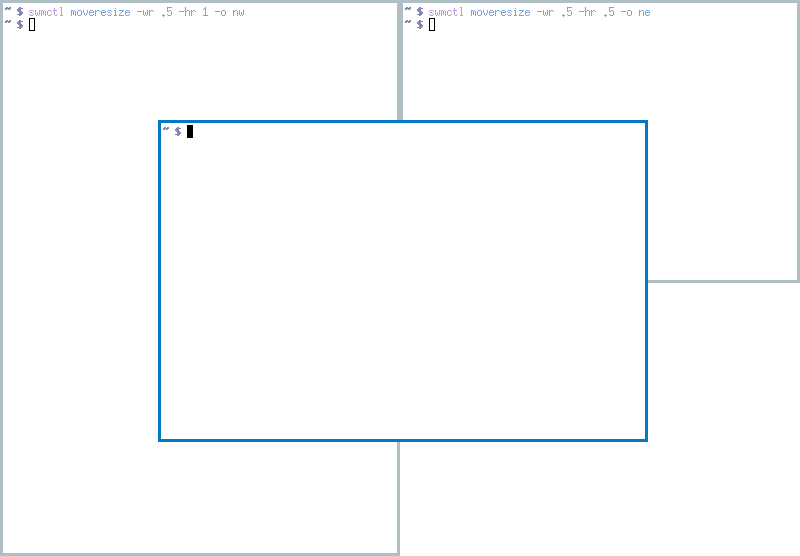
\includegraphics[width=10cm]{img/wins.png}
        \end{center}
    \end{frame}

    \begin{frame}{Architecture}
        \begin{itemize}
            \item no traditional config file, no keybindings
            \item swmrc -- startup shell script
            \item swmctl -- command line utility
            \item sxhkd, xdotool, wmctrl -- 3rd party tools
        \end{itemize}
        \begin{center}
            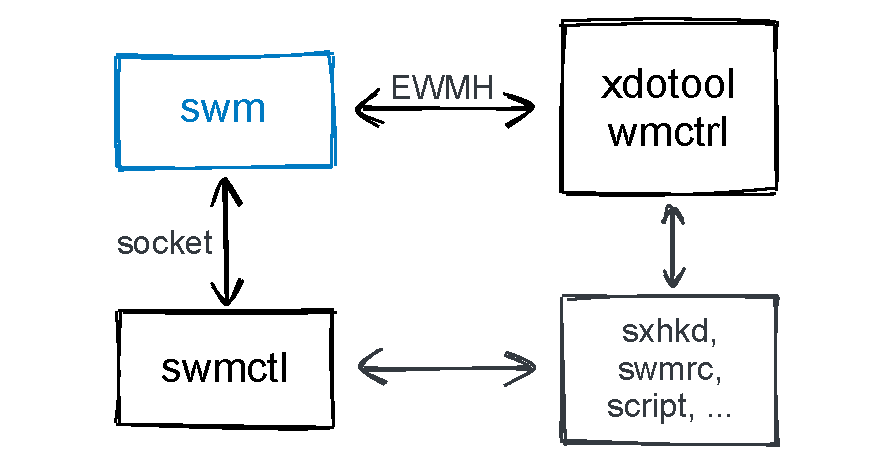
\includegraphics[width=8cm]{img/arch.pdf}
        \end{center}
    \end{frame}

    \begin{frame}{EWMH messages, swmctl commands}
        \codeblock{bash}{listings/xdotool.txt}
        \codeblock{bash}{listings/swmctl.txt}
        \codeblock{bash}{listings/swmctl2.txt}
    \end{frame}

    \begin{frame}[fragile]{Groups \small{(virtual desktops)}}
        \begin{itemize}
            \item Multiple groups visible simultaneously
            \item One window in multiple groups
        \end{itemize}
        \codeblock{bash}{listings/groups.txt}
        \begin{center}
            
\includegraphics[width=7cm]{../img/group_info.png}
        \end{center}
    \end{frame}

    \begin{frame}{Implementation}
        \begin{itemize}
            \item swm and swmctl written in Go
            \item integration tests
            \begin{itemize}
                \item custom shell script for headless testing (Xvfm)
            \end{itemize}
            \item published on GitHub under MIT license
        \end{itemize}
        \vspace{1cm}
        \url{https://github.com/janbina/swm}
        \begin{center}
            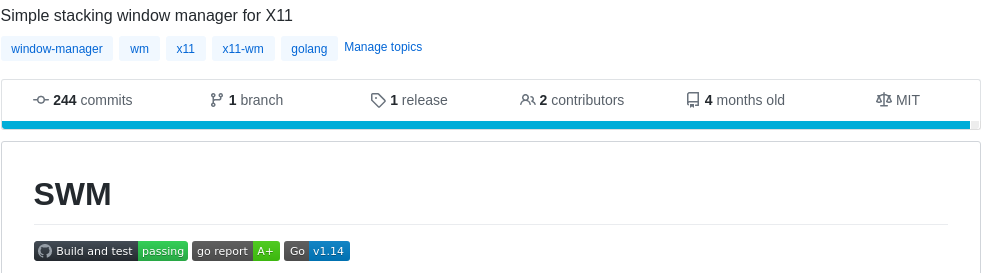
\includegraphics[width=12cm]{img/github.png}
        \end{center}
    \end{frame}

    % ============ Additional slides (thanks, refs, demo, ...) ============
    \backupbegin

    \begin{frame}
        \centering
        \Huge \textbf{Thanks for your attention} \\
        \vspace{30pt}
        \Huge \textbf{\textcolor{ctu}{Questions?}}
    \end{frame}

    \begin{frame}{References}
        \begin{itemize}
            \item sxhkd: \url{https://github.com/baskerville/sxhkd}
            \item xdotool: \url{https://github.com/jordansissel/xdotool}
            \item wmctrl: \url{http://tripie.sweb.cz/utils/wmctrl}
            \item cwm: \url{https://man.openbsd.org/cwm}
            \item i3: \url{https://i3wm.org}
        \end{itemize}
    \end{frame}

    \backupend

\end{document}
